\documentclass[11pt]{article}

    \usepackage[breakable]{tcolorbox}
    \usepackage{parskip} % Stop auto-indenting (to mimic markdown behaviour)
    

    % Basic figure setup, for now with no caption control since it's done
    % automatically by Pandoc (which extracts ![](path) syntax from Markdown).
    \usepackage{graphicx}
    % Keep aspect ratio if custom image width or height is specified
    \setkeys{Gin}{keepaspectratio}
    % Maintain compatibility with old templates. Remove in nbconvert 6.0
    \let\Oldincludegraphics\includegraphics
    % Ensure that by default, figures have no caption (until we provide a
    % proper Figure object with a Caption API and a way to capture that
    % in the conversion process - todo).
    \usepackage{caption}
    \DeclareCaptionFormat{nocaption}{}
    \captionsetup{format=nocaption,aboveskip=0pt,belowskip=0pt}

    \usepackage{float}
    \floatplacement{figure}{H} % forces figures to be placed at the correct location
    \usepackage{xcolor} % Allow colors to be defined
    \usepackage{enumerate} % Needed for markdown enumerations to work
    \usepackage{geometry} % Used to adjust the document margins
    \usepackage{amsmath} % Equations
    \usepackage{amssymb} % Equations
    \usepackage{textcomp} % defines textquotesingle
    % Hack from http://tex.stackexchange.com/a/47451/13684:
    \AtBeginDocument{%
        \def\PYZsq{\textquotesingle}% Upright quotes in Pygmentized code
    }
    \usepackage{upquote} % Upright quotes for verbatim code
    \usepackage{eurosym} % defines \euro

    \usepackage{iftex}
    \ifPDFTeX
        \usepackage[T1]{fontenc}
        \IfFileExists{alphabeta.sty}{
              \usepackage{alphabeta}
          }{
              \usepackage[mathletters]{ucs}
              \usepackage[utf8x]{inputenc}
          }
    \else
        \usepackage{fontspec}
        \usepackage{unicode-math}
    \fi

    \usepackage{fancyvrb} % verbatim replacement that allows latex
    \usepackage{grffile} % extends the file name processing of package graphics
                         % to support a larger range
    \makeatletter % fix for old versions of grffile with XeLaTeX
    \@ifpackagelater{grffile}{2019/11/01}
    {
      % Do nothing on new versions
    }
    {
      \def\Gread@@xetex#1{%
        \IfFileExists{"\Gin@base".bb}%
        {\Gread@eps{\Gin@base.bb}}%
        {\Gread@@xetex@aux#1}%
      }
    }
    \makeatother
    \usepackage[Export]{adjustbox} % Used to constrain images to a maximum size
    \adjustboxset{max size={0.9\linewidth}{0.9\paperheight}}

    % The hyperref package gives us a pdf with properly built
    % internal navigation ('pdf bookmarks' for the table of contents,
    % internal cross-reference links, web links for URLs, etc.)
    \usepackage{hyperref}
    % The default LaTeX title has an obnoxious amount of whitespace. By default,
    % titling removes some of it. It also provides customization options.
    \usepackage{titling}
    \usepackage{longtable} % longtable support required by pandoc >1.10
    \usepackage{booktabs}  % table support for pandoc > 1.12.2
    \usepackage{array}     % table support for pandoc >= 2.11.3
    \usepackage{calc}      % table minipage width calculation for pandoc >= 2.11.1
    \usepackage[inline]{enumitem} % IRkernel/repr support (it uses the enumerate* environment)
    \usepackage[normalem]{ulem} % ulem is needed to support strikethroughs (\sout)
                                % normalem makes italics be italics, not underlines
    \usepackage{soul}      % strikethrough (\st) support for pandoc >= 3.0.0
    \usepackage{mathrsfs}
    

    
    % Colors for the hyperref package
    \definecolor{urlcolor}{rgb}{0,.145,.698}
    \definecolor{linkcolor}{rgb}{.71,0.21,0.01}
    \definecolor{citecolor}{rgb}{.12,.54,.11}

    % ANSI colors
    \definecolor{ansi-black}{HTML}{3E424D}
    \definecolor{ansi-black-intense}{HTML}{282C36}
    \definecolor{ansi-red}{HTML}{E75C58}
    \definecolor{ansi-red-intense}{HTML}{B22B31}
    \definecolor{ansi-green}{HTML}{00A250}
    \definecolor{ansi-green-intense}{HTML}{007427}
    \definecolor{ansi-yellow}{HTML}{DDB62B}
    \definecolor{ansi-yellow-intense}{HTML}{B27D12}
    \definecolor{ansi-blue}{HTML}{208FFB}
    \definecolor{ansi-blue-intense}{HTML}{0065CA}
    \definecolor{ansi-magenta}{HTML}{D160C4}
    \definecolor{ansi-magenta-intense}{HTML}{A03196}
    \definecolor{ansi-cyan}{HTML}{60C6C8}
    \definecolor{ansi-cyan-intense}{HTML}{258F8F}
    \definecolor{ansi-white}{HTML}{C5C1B4}
    \definecolor{ansi-white-intense}{HTML}{A1A6B2}
    \definecolor{ansi-default-inverse-fg}{HTML}{FFFFFF}
    \definecolor{ansi-default-inverse-bg}{HTML}{000000}

    % common color for the border for error outputs.
    \definecolor{outerrorbackground}{HTML}{FFDFDF}

    % commands and environments needed by pandoc snippets
    % extracted from the output of `pandoc -s`
    \providecommand{\tightlist}{%
      \setlength{\itemsep}{0pt}\setlength{\parskip}{0pt}}
    \DefineVerbatimEnvironment{Highlighting}{Verbatim}{commandchars=\\\{\}}
    % Add ',fontsize=\small' for more characters per line
    \newenvironment{Shaded}{}{}
    \newcommand{\KeywordTok}[1]{\textcolor[rgb]{0.00,0.44,0.13}{\textbf{{#1}}}}
    \newcommand{\DataTypeTok}[1]{\textcolor[rgb]{0.56,0.13,0.00}{{#1}}}
    \newcommand{\DecValTok}[1]{\textcolor[rgb]{0.25,0.63,0.44}{{#1}}}
    \newcommand{\BaseNTok}[1]{\textcolor[rgb]{0.25,0.63,0.44}{{#1}}}
    \newcommand{\FloatTok}[1]{\textcolor[rgb]{0.25,0.63,0.44}{{#1}}}
    \newcommand{\CharTok}[1]{\textcolor[rgb]{0.25,0.44,0.63}{{#1}}}
    \newcommand{\StringTok}[1]{\textcolor[rgb]{0.25,0.44,0.63}{{#1}}}
    \newcommand{\CommentTok}[1]{\textcolor[rgb]{0.38,0.63,0.69}{\textit{{#1}}}}
    \newcommand{\OtherTok}[1]{\textcolor[rgb]{0.00,0.44,0.13}{{#1}}}
    \newcommand{\AlertTok}[1]{\textcolor[rgb]{1.00,0.00,0.00}{\textbf{{#1}}}}
    \newcommand{\FunctionTok}[1]{\textcolor[rgb]{0.02,0.16,0.49}{{#1}}}
    \newcommand{\RegionMarkerTok}[1]{{#1}}
    \newcommand{\ErrorTok}[1]{\textcolor[rgb]{1.00,0.00,0.00}{\textbf{{#1}}}}
    \newcommand{\NormalTok}[1]{{#1}}

    % Additional commands for more recent versions of Pandoc
    \newcommand{\ConstantTok}[1]{\textcolor[rgb]{0.53,0.00,0.00}{{#1}}}
    \newcommand{\SpecialCharTok}[1]{\textcolor[rgb]{0.25,0.44,0.63}{{#1}}}
    \newcommand{\VerbatimStringTok}[1]{\textcolor[rgb]{0.25,0.44,0.63}{{#1}}}
    \newcommand{\SpecialStringTok}[1]{\textcolor[rgb]{0.73,0.40,0.53}{{#1}}}
    \newcommand{\ImportTok}[1]{{#1}}
    \newcommand{\DocumentationTok}[1]{\textcolor[rgb]{0.73,0.13,0.13}{\textit{{#1}}}}
    \newcommand{\AnnotationTok}[1]{\textcolor[rgb]{0.38,0.63,0.69}{\textbf{\textit{{#1}}}}}
    \newcommand{\CommentVarTok}[1]{\textcolor[rgb]{0.38,0.63,0.69}{\textbf{\textit{{#1}}}}}
    \newcommand{\VariableTok}[1]{\textcolor[rgb]{0.10,0.09,0.49}{{#1}}}
    \newcommand{\ControlFlowTok}[1]{\textcolor[rgb]{0.00,0.44,0.13}{\textbf{{#1}}}}
    \newcommand{\OperatorTok}[1]{\textcolor[rgb]{0.40,0.40,0.40}{{#1}}}
    \newcommand{\BuiltInTok}[1]{{#1}}
    \newcommand{\ExtensionTok}[1]{{#1}}
    \newcommand{\PreprocessorTok}[1]{\textcolor[rgb]{0.74,0.48,0.00}{{#1}}}
    \newcommand{\AttributeTok}[1]{\textcolor[rgb]{0.49,0.56,0.16}{{#1}}}
    \newcommand{\InformationTok}[1]{\textcolor[rgb]{0.38,0.63,0.69}{\textbf{\textit{{#1}}}}}
    \newcommand{\WarningTok}[1]{\textcolor[rgb]{0.38,0.63,0.69}{\textbf{\textit{{#1}}}}}
    \makeatletter
    \newsavebox\pandoc@box
    \newcommand*\pandocbounded[1]{%
      \sbox\pandoc@box{#1}%
      % scaling factors for width and height
      \Gscale@div\@tempa\textheight{\dimexpr\ht\pandoc@box+\dp\pandoc@box\relax}%
      \Gscale@div\@tempb\linewidth{\wd\pandoc@box}%
      % select the smaller of both
      \ifdim\@tempb\p@<\@tempa\p@
        \let\@tempa\@tempb
      \fi
      % scaling accordingly (\@tempa < 1)
      \ifdim\@tempa\p@<\p@
        \scalebox{\@tempa}{\usebox\pandoc@box}%
      % scaling not needed, use as it is
      \else
        \usebox{\pandoc@box}%
      \fi
    }
    \makeatother

    % Define a nice break command that doesn't care if a line doesn't already
    % exist.
    \def\br{\hspace*{\fill} \\* }
    % Math Jax compatibility definitions
    \def\gt{>}
    \def\lt{<}
    \let\Oldtex\TeX
    \let\Oldlatex\LaTeX
    \renewcommand{\TeX}{\textrm{\Oldtex}}
    \renewcommand{\LaTeX}{\textrm{\Oldlatex}}
    % Document parameters
    % Document title
    \title{08\_notes}
    
    
    
    
    
    
    
% Pygments definitions
\makeatletter
\def\PY@reset{\let\PY@it=\relax \let\PY@bf=\relax%
    \let\PY@ul=\relax \let\PY@tc=\relax%
    \let\PY@bc=\relax \let\PY@ff=\relax}
\def\PY@tok#1{\csname PY@tok@#1\endcsname}
\def\PY@toks#1+{\ifx\relax#1\empty\else%
    \PY@tok{#1}\expandafter\PY@toks\fi}
\def\PY@do#1{\PY@bc{\PY@tc{\PY@ul{%
    \PY@it{\PY@bf{\PY@ff{#1}}}}}}}
\def\PY#1#2{\PY@reset\PY@toks#1+\relax+\PY@do{#2}}

\@namedef{PY@tok@w}{\def\PY@tc##1{\textcolor[rgb]{0.73,0.73,0.73}{##1}}}
\@namedef{PY@tok@c}{\let\PY@it=\textit\def\PY@tc##1{\textcolor[rgb]{0.24,0.48,0.48}{##1}}}
\@namedef{PY@tok@cp}{\def\PY@tc##1{\textcolor[rgb]{0.61,0.40,0.00}{##1}}}
\@namedef{PY@tok@k}{\let\PY@bf=\textbf\def\PY@tc##1{\textcolor[rgb]{0.00,0.50,0.00}{##1}}}
\@namedef{PY@tok@kp}{\def\PY@tc##1{\textcolor[rgb]{0.00,0.50,0.00}{##1}}}
\@namedef{PY@tok@kt}{\def\PY@tc##1{\textcolor[rgb]{0.69,0.00,0.25}{##1}}}
\@namedef{PY@tok@o}{\def\PY@tc##1{\textcolor[rgb]{0.40,0.40,0.40}{##1}}}
\@namedef{PY@tok@ow}{\let\PY@bf=\textbf\def\PY@tc##1{\textcolor[rgb]{0.67,0.13,1.00}{##1}}}
\@namedef{PY@tok@nb}{\def\PY@tc##1{\textcolor[rgb]{0.00,0.50,0.00}{##1}}}
\@namedef{PY@tok@nf}{\def\PY@tc##1{\textcolor[rgb]{0.00,0.00,1.00}{##1}}}
\@namedef{PY@tok@nc}{\let\PY@bf=\textbf\def\PY@tc##1{\textcolor[rgb]{0.00,0.00,1.00}{##1}}}
\@namedef{PY@tok@nn}{\let\PY@bf=\textbf\def\PY@tc##1{\textcolor[rgb]{0.00,0.00,1.00}{##1}}}
\@namedef{PY@tok@ne}{\let\PY@bf=\textbf\def\PY@tc##1{\textcolor[rgb]{0.80,0.25,0.22}{##1}}}
\@namedef{PY@tok@nv}{\def\PY@tc##1{\textcolor[rgb]{0.10,0.09,0.49}{##1}}}
\@namedef{PY@tok@no}{\def\PY@tc##1{\textcolor[rgb]{0.53,0.00,0.00}{##1}}}
\@namedef{PY@tok@nl}{\def\PY@tc##1{\textcolor[rgb]{0.46,0.46,0.00}{##1}}}
\@namedef{PY@tok@ni}{\let\PY@bf=\textbf\def\PY@tc##1{\textcolor[rgb]{0.44,0.44,0.44}{##1}}}
\@namedef{PY@tok@na}{\def\PY@tc##1{\textcolor[rgb]{0.41,0.47,0.13}{##1}}}
\@namedef{PY@tok@nt}{\let\PY@bf=\textbf\def\PY@tc##1{\textcolor[rgb]{0.00,0.50,0.00}{##1}}}
\@namedef{PY@tok@nd}{\def\PY@tc##1{\textcolor[rgb]{0.67,0.13,1.00}{##1}}}
\@namedef{PY@tok@s}{\def\PY@tc##1{\textcolor[rgb]{0.73,0.13,0.13}{##1}}}
\@namedef{PY@tok@sd}{\let\PY@it=\textit\def\PY@tc##1{\textcolor[rgb]{0.73,0.13,0.13}{##1}}}
\@namedef{PY@tok@si}{\let\PY@bf=\textbf\def\PY@tc##1{\textcolor[rgb]{0.64,0.35,0.47}{##1}}}
\@namedef{PY@tok@se}{\let\PY@bf=\textbf\def\PY@tc##1{\textcolor[rgb]{0.67,0.36,0.12}{##1}}}
\@namedef{PY@tok@sr}{\def\PY@tc##1{\textcolor[rgb]{0.64,0.35,0.47}{##1}}}
\@namedef{PY@tok@ss}{\def\PY@tc##1{\textcolor[rgb]{0.10,0.09,0.49}{##1}}}
\@namedef{PY@tok@sx}{\def\PY@tc##1{\textcolor[rgb]{0.00,0.50,0.00}{##1}}}
\@namedef{PY@tok@m}{\def\PY@tc##1{\textcolor[rgb]{0.40,0.40,0.40}{##1}}}
\@namedef{PY@tok@gh}{\let\PY@bf=\textbf\def\PY@tc##1{\textcolor[rgb]{0.00,0.00,0.50}{##1}}}
\@namedef{PY@tok@gu}{\let\PY@bf=\textbf\def\PY@tc##1{\textcolor[rgb]{0.50,0.00,0.50}{##1}}}
\@namedef{PY@tok@gd}{\def\PY@tc##1{\textcolor[rgb]{0.63,0.00,0.00}{##1}}}
\@namedef{PY@tok@gi}{\def\PY@tc##1{\textcolor[rgb]{0.00,0.52,0.00}{##1}}}
\@namedef{PY@tok@gr}{\def\PY@tc##1{\textcolor[rgb]{0.89,0.00,0.00}{##1}}}
\@namedef{PY@tok@ge}{\let\PY@it=\textit}
\@namedef{PY@tok@gs}{\let\PY@bf=\textbf}
\@namedef{PY@tok@ges}{\let\PY@bf=\textbf\let\PY@it=\textit}
\@namedef{PY@tok@gp}{\let\PY@bf=\textbf\def\PY@tc##1{\textcolor[rgb]{0.00,0.00,0.50}{##1}}}
\@namedef{PY@tok@go}{\def\PY@tc##1{\textcolor[rgb]{0.44,0.44,0.44}{##1}}}
\@namedef{PY@tok@gt}{\def\PY@tc##1{\textcolor[rgb]{0.00,0.27,0.87}{##1}}}
\@namedef{PY@tok@err}{\def\PY@bc##1{{\setlength{\fboxsep}{\string -\fboxrule}\fcolorbox[rgb]{1.00,0.00,0.00}{1,1,1}{\strut ##1}}}}
\@namedef{PY@tok@kc}{\let\PY@bf=\textbf\def\PY@tc##1{\textcolor[rgb]{0.00,0.50,0.00}{##1}}}
\@namedef{PY@tok@kd}{\let\PY@bf=\textbf\def\PY@tc##1{\textcolor[rgb]{0.00,0.50,0.00}{##1}}}
\@namedef{PY@tok@kn}{\let\PY@bf=\textbf\def\PY@tc##1{\textcolor[rgb]{0.00,0.50,0.00}{##1}}}
\@namedef{PY@tok@kr}{\let\PY@bf=\textbf\def\PY@tc##1{\textcolor[rgb]{0.00,0.50,0.00}{##1}}}
\@namedef{PY@tok@bp}{\def\PY@tc##1{\textcolor[rgb]{0.00,0.50,0.00}{##1}}}
\@namedef{PY@tok@fm}{\def\PY@tc##1{\textcolor[rgb]{0.00,0.00,1.00}{##1}}}
\@namedef{PY@tok@vc}{\def\PY@tc##1{\textcolor[rgb]{0.10,0.09,0.49}{##1}}}
\@namedef{PY@tok@vg}{\def\PY@tc##1{\textcolor[rgb]{0.10,0.09,0.49}{##1}}}
\@namedef{PY@tok@vi}{\def\PY@tc##1{\textcolor[rgb]{0.10,0.09,0.49}{##1}}}
\@namedef{PY@tok@vm}{\def\PY@tc##1{\textcolor[rgb]{0.10,0.09,0.49}{##1}}}
\@namedef{PY@tok@sa}{\def\PY@tc##1{\textcolor[rgb]{0.73,0.13,0.13}{##1}}}
\@namedef{PY@tok@sb}{\def\PY@tc##1{\textcolor[rgb]{0.73,0.13,0.13}{##1}}}
\@namedef{PY@tok@sc}{\def\PY@tc##1{\textcolor[rgb]{0.73,0.13,0.13}{##1}}}
\@namedef{PY@tok@dl}{\def\PY@tc##1{\textcolor[rgb]{0.73,0.13,0.13}{##1}}}
\@namedef{PY@tok@s2}{\def\PY@tc##1{\textcolor[rgb]{0.73,0.13,0.13}{##1}}}
\@namedef{PY@tok@sh}{\def\PY@tc##1{\textcolor[rgb]{0.73,0.13,0.13}{##1}}}
\@namedef{PY@tok@s1}{\def\PY@tc##1{\textcolor[rgb]{0.73,0.13,0.13}{##1}}}
\@namedef{PY@tok@mb}{\def\PY@tc##1{\textcolor[rgb]{0.40,0.40,0.40}{##1}}}
\@namedef{PY@tok@mf}{\def\PY@tc##1{\textcolor[rgb]{0.40,0.40,0.40}{##1}}}
\@namedef{PY@tok@mh}{\def\PY@tc##1{\textcolor[rgb]{0.40,0.40,0.40}{##1}}}
\@namedef{PY@tok@mi}{\def\PY@tc##1{\textcolor[rgb]{0.40,0.40,0.40}{##1}}}
\@namedef{PY@tok@il}{\def\PY@tc##1{\textcolor[rgb]{0.40,0.40,0.40}{##1}}}
\@namedef{PY@tok@mo}{\def\PY@tc##1{\textcolor[rgb]{0.40,0.40,0.40}{##1}}}
\@namedef{PY@tok@ch}{\let\PY@it=\textit\def\PY@tc##1{\textcolor[rgb]{0.24,0.48,0.48}{##1}}}
\@namedef{PY@tok@cm}{\let\PY@it=\textit\def\PY@tc##1{\textcolor[rgb]{0.24,0.48,0.48}{##1}}}
\@namedef{PY@tok@cpf}{\let\PY@it=\textit\def\PY@tc##1{\textcolor[rgb]{0.24,0.48,0.48}{##1}}}
\@namedef{PY@tok@c1}{\let\PY@it=\textit\def\PY@tc##1{\textcolor[rgb]{0.24,0.48,0.48}{##1}}}
\@namedef{PY@tok@cs}{\let\PY@it=\textit\def\PY@tc##1{\textcolor[rgb]{0.24,0.48,0.48}{##1}}}

\def\PYZbs{\char`\\}
\def\PYZus{\char`\_}
\def\PYZob{\char`\{}
\def\PYZcb{\char`\}}
\def\PYZca{\char`\^}
\def\PYZam{\char`\&}
\def\PYZlt{\char`\<}
\def\PYZgt{\char`\>}
\def\PYZsh{\char`\#}
\def\PYZpc{\char`\%}
\def\PYZdl{\char`\$}
\def\PYZhy{\char`\-}
\def\PYZsq{\char`\'}
\def\PYZdq{\char`\"}
\def\PYZti{\char`\~}
% for compatibility with earlier versions
\def\PYZat{@}
\def\PYZlb{[}
\def\PYZrb{]}
\makeatother


    % For linebreaks inside Verbatim environment from package fancyvrb.
    \makeatletter
        \newbox\Wrappedcontinuationbox
        \newbox\Wrappedvisiblespacebox
        \newcommand*\Wrappedvisiblespace {\textcolor{red}{\textvisiblespace}}
        \newcommand*\Wrappedcontinuationsymbol {\textcolor{red}{\llap{\tiny$\m@th\hookrightarrow$}}}
        \newcommand*\Wrappedcontinuationindent {3ex }
        \newcommand*\Wrappedafterbreak {\kern\Wrappedcontinuationindent\copy\Wrappedcontinuationbox}
        % Take advantage of the already applied Pygments mark-up to insert
        % potential linebreaks for TeX processing.
        %        {, <, #, %, $, ' and ": go to next line.
        %        _, }, ^, &, >, - and ~: stay at end of broken line.
        % Use of \textquotesingle for straight quote.
        \newcommand*\Wrappedbreaksatspecials {%
            \def\PYGZus{\discretionary{\char`\_}{\Wrappedafterbreak}{\char`\_}}%
            \def\PYGZob{\discretionary{}{\Wrappedafterbreak\char`\{}{\char`\{}}%
            \def\PYGZcb{\discretionary{\char`\}}{\Wrappedafterbreak}{\char`\}}}%
            \def\PYGZca{\discretionary{\char`\^}{\Wrappedafterbreak}{\char`\^}}%
            \def\PYGZam{\discretionary{\char`\&}{\Wrappedafterbreak}{\char`\&}}%
            \def\PYGZlt{\discretionary{}{\Wrappedafterbreak\char`\<}{\char`\<}}%
            \def\PYGZgt{\discretionary{\char`\>}{\Wrappedafterbreak}{\char`\>}}%
            \def\PYGZsh{\discretionary{}{\Wrappedafterbreak\char`\#}{\char`\#}}%
            \def\PYGZpc{\discretionary{}{\Wrappedafterbreak\char`\%}{\char`\%}}%
            \def\PYGZdl{\discretionary{}{\Wrappedafterbreak\char`\$}{\char`\$}}%
            \def\PYGZhy{\discretionary{\char`\-}{\Wrappedafterbreak}{\char`\-}}%
            \def\PYGZsq{\discretionary{}{\Wrappedafterbreak\textquotesingle}{\textquotesingle}}%
            \def\PYGZdq{\discretionary{}{\Wrappedafterbreak\char`\"}{\char`\"}}%
            \def\PYGZti{\discretionary{\char`\~}{\Wrappedafterbreak}{\char`\~}}%
        }
        % Some characters . , ; ? ! / are not pygmentized.
        % This macro makes them "active" and they will insert potential linebreaks
        \newcommand*\Wrappedbreaksatpunct {%
            \lccode`\~`\.\lowercase{\def~}{\discretionary{\hbox{\char`\.}}{\Wrappedafterbreak}{\hbox{\char`\.}}}%
            \lccode`\~`\,\lowercase{\def~}{\discretionary{\hbox{\char`\,}}{\Wrappedafterbreak}{\hbox{\char`\,}}}%
            \lccode`\~`\;\lowercase{\def~}{\discretionary{\hbox{\char`\;}}{\Wrappedafterbreak}{\hbox{\char`\;}}}%
            \lccode`\~`\:\lowercase{\def~}{\discretionary{\hbox{\char`\:}}{\Wrappedafterbreak}{\hbox{\char`\:}}}%
            \lccode`\~`\?\lowercase{\def~}{\discretionary{\hbox{\char`\?}}{\Wrappedafterbreak}{\hbox{\char`\?}}}%
            \lccode`\~`\!\lowercase{\def~}{\discretionary{\hbox{\char`\!}}{\Wrappedafterbreak}{\hbox{\char`\!}}}%
            \lccode`\~`\/\lowercase{\def~}{\discretionary{\hbox{\char`\/}}{\Wrappedafterbreak}{\hbox{\char`\/}}}%
            \catcode`\.\active
            \catcode`\,\active
            \catcode`\;\active
            \catcode`\:\active
            \catcode`\?\active
            \catcode`\!\active
            \catcode`\/\active
            \lccode`\~`\~
        }
    \makeatother

    \let\OriginalVerbatim=\Verbatim
    \makeatletter
    \renewcommand{\Verbatim}[1][1]{%
        %\parskip\z@skip
        \sbox\Wrappedcontinuationbox {\Wrappedcontinuationsymbol}%
        \sbox\Wrappedvisiblespacebox {\FV@SetupFont\Wrappedvisiblespace}%
        \def\FancyVerbFormatLine ##1{\hsize\linewidth
            \vtop{\raggedright\hyphenpenalty\z@\exhyphenpenalty\z@
                \doublehyphendemerits\z@\finalhyphendemerits\z@
                \strut ##1\strut}%
        }%
        % If the linebreak is at a space, the latter will be displayed as visible
        % space at end of first line, and a continuation symbol starts next line.
        % Stretch/shrink are however usually zero for typewriter font.
        \def\FV@Space {%
            \nobreak\hskip\z@ plus\fontdimen3\font minus\fontdimen4\font
            \discretionary{\copy\Wrappedvisiblespacebox}{\Wrappedafterbreak}
            {\kern\fontdimen2\font}%
        }%

        % Allow breaks at special characters using \PYG... macros.
        \Wrappedbreaksatspecials
        % Breaks at punctuation characters . , ; ? ! and / need catcode=\active
        \OriginalVerbatim[#1,codes*=\Wrappedbreaksatpunct]%
    }
    \makeatother

    % Exact colors from NB
    \definecolor{incolor}{HTML}{303F9F}
    \definecolor{outcolor}{HTML}{D84315}
    \definecolor{cellborder}{HTML}{CFCFCF}
    \definecolor{cellbackground}{HTML}{F7F7F7}

    % prompt
    \makeatletter
    \newcommand{\boxspacing}{\kern\kvtcb@left@rule\kern\kvtcb@boxsep}
    \makeatother
    \newcommand{\prompt}[4]{
        {\ttfamily\llap{{\color{#2}[#3]:\hspace{3pt}#4}}\vspace{-\baselineskip}}
    }
    

    
    % Prevent overflowing lines due to hard-to-break entities
    \sloppy
    % Setup hyperref package
    \hypersetup{
      breaklinks=true,  % so long urls are correctly broken across lines
      colorlinks=true,
      urlcolor=urlcolor,
      linkcolor=linkcolor,
      citecolor=citecolor,
      }
    % Slightly bigger margins than the latex defaults
    
    \geometry{verbose,tmargin=1in,bmargin=1in,lmargin=1in,rmargin=1in}
    
    

\begin{document}
    
    \maketitle
    
    

    
    \section{Week 8 - Notes: Oscillators and Modeling
Oscillations}\label{week-8---notes-oscillators-and-modeling-oscillations}

We continue our study of physics phenomena that exhibits recurrent or
periodic behavior. Some systems repeat their motion in a regular
pattern, and we call them oscillators.

We have met this behavior many times. This is because we often look at
the behavior of stems just a little bit away from equilibrium. Systems
with local stable equilibria will have oscillatory behavior in a region
around that equilibrium point. Note below the made up example of a
potential energy function that has local minima and maxima.

Near the local minima, the system will oscillate back and forth. The
potential energy function will look like a parabola.

    \begin{tcolorbox}[breakable, size=fbox, boxrule=1pt, pad at break*=1mm,colback=cellbackground, colframe=cellborder]
\prompt{In}{incolor}{18}{\boxspacing}
\begin{Verbatim}[commandchars=\\\{\}]
\PY{c+c1}{\PYZsh{}\PYZsh{} Make a plot of a potential energy function with 3 local minima}

\PY{k+kn}{import}\PY{+w}{ }\PY{n+nn}{numpy}\PY{+w}{ }\PY{k}{as}\PY{+w}{ }\PY{n+nn}{np}
\PY{k+kn}{import}\PY{+w}{ }\PY{n+nn}{matplotlib}\PY{n+nn}{.}\PY{n+nn}{pyplot}\PY{+w}{ }\PY{k}{as}\PY{+w}{ }\PY{n+nn}{plt}
\PY{n}{plt}\PY{o}{.}\PY{n}{style}\PY{o}{.}\PY{n}{use}\PY{p}{(}\PY{l+s+s1}{\PYZsq{}}\PY{l+s+s1}{seaborn\PYZhy{}v0\PYZus{}8\PYZhy{}colorblind}\PY{l+s+s1}{\PYZsq{}}\PY{p}{)}

\PY{n}{x} \PY{o}{=} \PY{n}{np}\PY{o}{.}\PY{n}{linspace}\PY{p}{(}\PY{o}{\PYZhy{}}\PY{l+m+mi}{2}\PY{p}{,} \PY{l+m+mi}{2}\PY{p}{,} \PY{l+m+mi}{100}\PY{p}{)}
\PY{n}{U} \PY{o}{=} \PY{n}{x}\PY{o}{*}\PY{o}{*}\PY{l+m+mi}{6} \PY{o}{\PYZhy{}} \PY{l+m+mi}{2}\PY{o}{*}\PY{n}{x}\PY{o}{*}\PY{o}{*}\PY{l+m+mi}{3} \PY{o}{\PYZhy{}} \PY{l+m+mi}{10}\PY{o}{*}\PY{n}{x}\PY{o}{*}\PY{o}{*}\PY{l+m+mi}{2} \PY{o}{+} \PY{n}{x}

\PY{n}{plt}\PY{o}{.}\PY{n}{plot}\PY{p}{(}\PY{n}{x}\PY{p}{,} \PY{n}{U}\PY{p}{)}
\PY{n}{plt}\PY{o}{.}\PY{n}{xlabel}\PY{p}{(}\PY{l+s+s1}{\PYZsq{}}\PY{l+s+s1}{x}\PY{l+s+s1}{\PYZsq{}}\PY{p}{)}
\PY{n}{plt}\PY{o}{.}\PY{n}{ylabel}\PY{p}{(}\PY{l+s+s1}{\PYZsq{}}\PY{l+s+s1}{Potential Energy}\PY{l+s+s1}{\PYZsq{}}\PY{p}{)}
\PY{n}{plt}\PY{o}{.}\PY{n}{title}\PY{p}{(}\PY{l+s+s1}{\PYZsq{}}\PY{l+s+s1}{Potential Energy Function}\PY{l+s+s1}{\PYZsq{}}\PY{p}{)}
\PY{n}{plt}\PY{o}{.}\PY{n}{grid}\PY{p}{(}\PY{k+kc}{True}\PY{p}{)}
\PY{n}{plt}\PY{o}{.}\PY{n}{tight\PYZus{}layout}\PY{p}{(}\PY{p}{)}
\PY{n}{plt}\PY{o}{.}\PY{n}{show}\PY{p}{(}\PY{p}{)}
\end{Verbatim}
\end{tcolorbox}

    \begin{center}
    \adjustimage{max size={0.9\linewidth}{0.9\paperheight}}{08_notes_files/08_notes_1_0.png}
    \end{center}
    { \hspace*{\fill} \\}
    
    \subsection{Why do we often see oscillations in
physics?}\label{why-do-we-often-see-oscillations-in-physics}

Oscillatory behavior is common in physics because many systems have a
stable equilibrium point. When we disturb the system from equilibrium,
it will oscillate back and forth around that equilibrium point. Let's
assume there's a given stable equilibrium point at \(x=a\), we can write
the potential energy function as a Taylor series expansion around that
point:

\[U(x) \approx U(a) + \dfrac{dU}{dx}\bigg|_{x=a}(x-a) + \dfrac{1}{2}\dfrac{d^2U}{dx^2}\bigg|_{x=a}(x-a)^2 + \cdots\]

The linear term is zero because the equilibrium point is a minimum,
\(\dfrac{dU}{dx}\bigg|_{x=a}=0\). The quadratic term is remains as does
the constant term. So up to the quadratic term, the potential energy
function is a parabola.

\[U(x) \approx U(a) + \dfrac{1}{2}\dfrac{d^2U}{dx^2}\bigg|_{x=a}(x-a)^2\]

We can write the value of the second derivative as a constant \(k\). It
will just be the measure of the concavity of the potential energy
function at the equilibrium point. So near \(x=a\), the potential energy
function will look like a parabola of the form:

\[U(x) \approx U(a) + \dfrac{1}{2}k(x-a)^2\]

Because only changes in potential energy are important, we can ignore
the constant term \(U(a)\). The change in potential energy is then:

\[\Delta U = \dfrac{1}{2}k(x_f-a)^2 - \dfrac{1}{2}k(x_i-a)^2\]
\[\Delta U = U_f - U_i\]

This is just the change in potential energy for any spring-mass system
(any SHO) if \(k>0\).

    \subsection{The Exact Solution for the Simple Harmonic
Oscillator}\label{the-exact-solution-for-the-simple-harmonic-oscillator}

This potential \(U=\frac{1}{2}kx^2\) is the potential for the simple
harmonic oscillator when \(k>0\) and we are modeling around a stable
critical point. We know that this potential energy will produce a
restoring force.

\[F = -\dfrac{dU}{dx} = -kx\]

Thus our equation of motion is:

\[m\ddot{x} = -kx,\]

Or

\[\ddot{x} = -\dfrac{k}{m}x.\]

The natural oscillation frequency of the SHO is:

\[\omega = \sqrt{\dfrac{k}{m}}.\]

And thus we obtain several forms of their general solution:

\[x(t) = A\cos(\omega t) + B\sin(\omega t)\]
\[x(t) = C\cos(\omega t + \phi)\] \[x(t) = D\sin(\omega t + \phi)\]

Where \(A\), \(B\), \(C\), \(D\), and \(\phi\) are constants that depend
on the initial conditions of the system. The phase \(\phi\) is the phase
angle of the oscillation. Each solution is equivalent to the others and
can be written as the other form. And each solution has two arbitrary
constants that depend on the initial conditions of the system.

\subsubsection{Complex forms of the SHO
solution}\label{complex-forms-of-the-sho-solution}

These forms are useful, but often lead to more complex algebra. We can
write the solution in terms of complex exponentials, which have the
advantage of simplifying the algebra. Let's try a complex form of the
solution:

\[x(t) = e^{i\omega t}\;\textrm{where}\;i^2=-1\]

Take its derivatives:

\[\dot{x}(t) = i\omega e^{i\omega t}\]
\[\ddot{x}(t) = (i\omega)(i\omega) e^{i\omega t} = -\omega^2 e^{i\omega t} = -\omega^2 x(t)\]

Note that \(e^{-i\omega t}\) is also a solution to the differential
equation that will produce this same result. So the general solution is
the linear combination of these two solutions:

\[x(t) = C_1 e^{i\omega t} + C_2 e^{-i\omega t}\]

where \(C_1\) and \(C_2\) are constants that depend on the initial
conditions of the system and \textbf{can be complex}. We still have two
arbitrary constants that depend on the initial conditions of the system,
which is needed for a second-order differential equation.

\subsubsection{But the solution to the motion of the SHO is
real!}\label{but-the-solution-to-the-motion-of-the-sho-is-real}

Yes, that is true. The solution must be a real function of time. This
puts conditions on the constants \(C_1\) and \(C_2\). Using the Euler
formula:

\[e^{i\theta} = \cos(\theta) + i\sin(\theta)\]

we can apply this to the functional form of the solution, such that,

\[e^{\pm i\omega t} = \cos(\omega t) \pm i\sin(\omega t).\]

Applying this to the general solution:

\[x(t) = C_1(\cos(\omega t) + i\sin(\omega t)) + C_2(\cos(\omega t) - i\sin(\omega t))\]
\[x(t) = (C_1 + C_2)\cos(\omega t) + i(C_1 - C_2)\sin(\omega t).\]

We grouped the terms in the last line to define some constants \(B_1\)
and \(B_2\):

\[B_1 = C_1 + C_2\] \[B_2 = i(C_1 - C_2)\]

So that,

\[x(t) = B_1\cos(\omega t) + B_2\sin(\omega t).\]

But \(B_1\) and \(B_2\) must be real because the rest of the solution is
real. What does that mean? Let's write \(C_1\) and \(C_2\) in terms of
\(B_1\) and \(B_2\):

\[C_1 = \dfrac{1}{2}\left(B_1-iB_2\right)\]
\[C_2 = \dfrac{1}{2}\left(B_1+iB_2\right)\]

    \subsection{Complex Conjugates}\label{complex-conjugates}

These values of \(C_1\) and \(C_2\) are the complex conjugates of each
other. The complex conjugate of a complex number \(z=a+ib\) is
\(z^*=a-ib\). The complex conjugate of a complex number is the same as
the original number, but with the sign of the imaginary part reversed.

We can draw these in the complex plane where the \(x\)-axis is the real
part and the \(y\)-axis is the imaginary part.

\begin{figure}
\centering
\pandocbounded{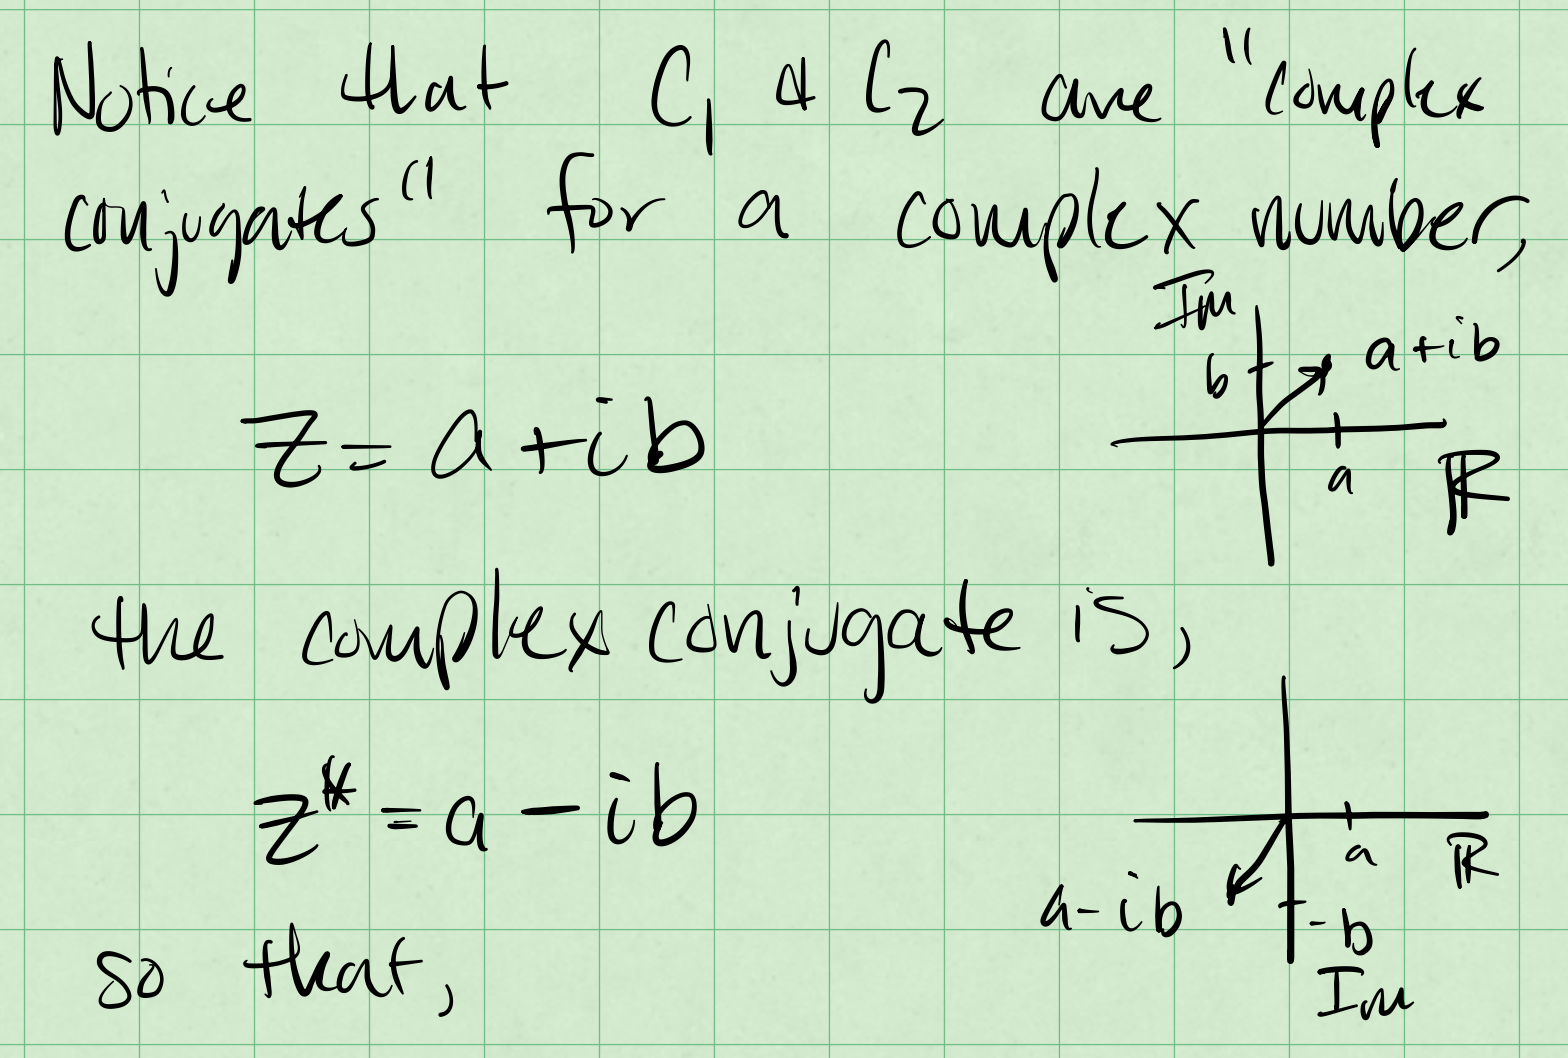
\includegraphics[keepaspectratio,alt={Complex Conjugates}]{/Users/caballero/repos/teaching/modern-classical-mechanics/content/images/notes/week8/conjugates_graph.png}}
\caption{Complex Conjugates}
\end{figure}

In the graph we can see that the complex conjugates are a reflection of
each other. This is because the imaginary part of the complex conjugate
is the negative of the original imaginary part.

The mathematics is quite useful for us. Consider the produce of two
complex conjugates:

\[z = a + ib\] \[z^* = a - ib\]

So that,

\[zz^* = (a+ib)(a-ib) = a^2 + b^2\]

The product of a complex number and its complex conjugate is always a
real number. Moreover, we can define the magnitude of a complex number
as:

\[|z| = \sqrt{zz^*} = \sqrt{a^2 + b^2},m\]

which is also real! Given that \(C_1\) and \(C_2\) are complex
conjugates (\(C_2 = C_1^*\)), we can write the general solution to the
SHO as:

\[x(t) = C_1 e^{i\omega t} + C_1^* e^{-i\omega t}\]

\subsubsection{What does that mean for the
SHO?}\label{what-does-that-mean-for-the-sho}

There's a few more mathematical properties for complex conjugates that
are useful for the SHO. The general solution to the SHO is. Let:

\[z = a + ib\] \[z^* = a - ib\]

So that,

\[z+z^* = 2a,\] \[z-z^* = 2ib.\]

We denote the Real Part of a complex number as \(Re(z)\) and the
Imaginary Part as \(Im(z)\). So that,

\[Re(z) = Re(z^*) = a,\] \[Im(z) = -Im(z^*) = b.\]

The real and imaginary parts of a complex number are real numbers. We
can apply these properties to the general solution of the SHO:

\[x(t) = C_1 e^{i\omega t} + C_1^* e^{-i\omega t}\]
\[x(t) = C_1 e^{i\omega t} + \left(C_1 e^{i\omega t}\right)^*\]
\[x(t) = 2Re\left(C_1 e^{i\omega t}\right)\]

let \(C = 2C_1\) so that,

\[x(t) = Re\left(C e^{i\omega t}\right).\]

This must be equal to a real function of time. For example,

\[x(t)= A\cos(\omega t-\delta),\]

which we can write as,

\[x(t) = Re\left(Ae^{i(\omega t - \delta)}\right) = Re\left(Ae^{-i\delta}e^{i\omega t}\right).\]

Thus,

\[C = Ae^{-i\delta}.\]

    This is a bit abstract, but let's try to graph this and make it a bit
concrete. Below, we've plotted the solution to an oscillator that starts
with a \(\delta = \pi/4\) phase shift. The solution is plotted in the
complex plane with rainbow colors to demonstrate time (from violet to
red). The starting point is marked with a black square, and because the
\(omega\) is positive, the solution moves counter-clockwise in the
plane.

Below that we trace the real part of the solution in the \(t\)-\(x\)
plane. This is not the same as a readout on something like an
oscilloscope, or a time trace of the solution. But we can rotate the
graph to be in the \(x\)-\(t\) plane - and thus a real temporal
solution. In all cases, the black square marks the starting point of the
solution, and the rainbow of points marks the solution as it moves in
time.

    \begin{tcolorbox}[breakable, size=fbox, boxrule=1pt, pad at break*=1mm,colback=cellbackground, colframe=cellborder]
\prompt{In}{incolor}{33}{\boxspacing}
\begin{Verbatim}[commandchars=\\\{\}]
\PY{k+kn}{import}\PY{+w}{ }\PY{n+nn}{numpy}\PY{+w}{ }\PY{k}{as}\PY{+w}{ }\PY{n+nn}{np}
\PY{k+kn}{import}\PY{+w}{ }\PY{n+nn}{matplotlib}\PY{n+nn}{.}\PY{n+nn}{pyplot}\PY{+w}{ }\PY{k}{as}\PY{+w}{ }\PY{n+nn}{plt}
\PY{k+kn}{from}\PY{+w}{ }\PY{n+nn}{matplotlib}\PY{+w}{ }\PY{k+kn}{import} \PY{n}{cm}

\PY{n}{plt}\PY{o}{.}\PY{n}{style}\PY{o}{.}\PY{n}{use}\PY{p}{(}\PY{l+s+s1}{\PYZsq{}}\PY{l+s+s1}{seaborn\PYZhy{}v0\PYZus{}8\PYZhy{}colorblind}\PY{l+s+s1}{\PYZsq{}}\PY{p}{)}

\PY{n}{C1} \PY{o}{=} \PY{l+m+mi}{1}
\PY{n}{delta} \PY{o}{=} \PY{n}{np}\PY{o}{.}\PY{n}{pi}\PY{o}{/}\PY{l+m+mi}{4}
\PY{n}{omega} \PY{o}{=} \PY{l+m+mi}{1}
\PY{n}{t} \PY{o}{=} \PY{n}{np}\PY{o}{.}\PY{n}{linspace}\PY{p}{(}\PY{l+m+mi}{0}\PY{p}{,} \PY{l+m+mi}{2}\PY{o}{*}\PY{n}{np}\PY{o}{.}\PY{n}{pi}\PY{p}{,} \PY{l+m+mi}{100}\PY{p}{)}

\PY{n}{x} \PY{o}{=} \PY{n}{C1}\PY{o}{*}\PY{n}{np}\PY{o}{.}\PY{n}{exp}\PY{p}{(}\PY{l+m+mi}{1}\PY{n}{j}\PY{o}{*}\PY{p}{(}\PY{n}{omega}\PY{o}{*}\PY{n}{t} \PY{o}{\PYZhy{}} \PY{n}{delta}\PY{p}{)}\PY{p}{)}

\PY{c+c1}{\PYZsh{}\PYZsh{} Plot the trajectory in the complex plane}

\PY{n}{fig}\PY{p}{,} \PY{n}{ax} \PY{o}{=} \PY{n}{plt}\PY{o}{.}\PY{n}{subplots}\PY{p}{(}\PY{l+m+mi}{1}\PY{p}{,}\PY{l+m+mi}{1}\PY{p}{,} \PY{n}{figsize}\PY{o}{=}\PY{p}{(}\PY{l+m+mi}{6}\PY{p}{,} \PY{l+m+mi}{6}\PY{p}{)}\PY{p}{)}
\PY{n}{plt}\PY{o}{.}\PY{n}{scatter}\PY{p}{(}\PY{n}{x}\PY{o}{.}\PY{n}{real}\PY{p}{,} \PY{n}{x}\PY{o}{.}\PY{n}{imag}\PY{p}{,} \PY{n}{c}\PY{o}{=}\PY{n}{t}\PY{p}{,} \PY{n}{cmap}\PY{o}{=}\PY{n}{cm}\PY{o}{.}\PY{n}{rainbow}\PY{p}{,} \PY{n}{s}\PY{o}{=}\PY{l+m+mi}{15}\PY{p}{)}
\PY{n}{plt}\PY{o}{.}\PY{n}{plot}\PY{p}{(}\PY{n}{x}\PY{o}{.}\PY{n}{real}\PY{p}{[}\PY{l+m+mi}{0}\PY{p}{]}\PY{p}{,} \PY{n}{x}\PY{o}{.}\PY{n}{imag}\PY{p}{[}\PY{l+m+mi}{0}\PY{p}{]}\PY{p}{,} \PY{l+s+s1}{\PYZsq{}}\PY{l+s+s1}{ks}\PY{l+s+s1}{\PYZsq{}}\PY{p}{,} \PY{n}{markersize}\PY{o}{=}\PY{l+m+mi}{15}\PY{p}{,} \PY{n}{label}\PY{o}{=}\PY{l+s+s1}{\PYZsq{}}\PY{l+s+s1}{Start}\PY{l+s+s1}{\PYZsq{}}\PY{p}{)}
\PY{n}{plt}\PY{o}{.}\PY{n}{axhline}\PY{p}{(}\PY{l+m+mi}{0}\PY{p}{,} \PY{n}{color}\PY{o}{=}\PY{l+s+s1}{\PYZsq{}}\PY{l+s+s1}{k}\PY{l+s+s1}{\PYZsq{}}\PY{p}{,} \PY{n}{lw}\PY{o}{=}\PY{l+m+mi}{2}\PY{p}{)}
\PY{n}{plt}\PY{o}{.}\PY{n}{axvline}\PY{p}{(}\PY{l+m+mi}{0}\PY{p}{,} \PY{n}{color}\PY{o}{=}\PY{l+s+s1}{\PYZsq{}}\PY{l+s+s1}{k}\PY{l+s+s1}{\PYZsq{}}\PY{p}{,} \PY{n}{lw}\PY{o}{=}\PY{l+m+mi}{2}\PY{p}{)}
\PY{n}{plt}\PY{o}{.}\PY{n}{grid}\PY{p}{(}\PY{p}{)}
\PY{n}{plt}\PY{o}{.}\PY{n}{xlabel}\PY{p}{(}\PY{l+s+s1}{\PYZsq{}}\PY{l+s+s1}{Real Part}\PY{l+s+s1}{\PYZsq{}}\PY{p}{)}
\PY{n}{plt}\PY{o}{.}\PY{n}{ylabel}\PY{p}{(}\PY{l+s+s1}{\PYZsq{}}\PY{l+s+s1}{Imaginary Part}\PY{l+s+s1}{\PYZsq{}}\PY{p}{)}
\PY{n}{plt}\PY{o}{.}\PY{n}{tight\PYZus{}layout}\PY{p}{(}\PY{p}{)}

\PY{c+c1}{\PYZsh{}\PYZsh{} Plot the trajectory in the t\PYZhy{}x plane}
\PY{n}{fig}\PY{p}{,} \PY{n}{ax} \PY{o}{=} \PY{n}{plt}\PY{o}{.}\PY{n}{subplots}\PY{p}{(}\PY{l+m+mi}{1}\PY{p}{,}\PY{l+m+mi}{1}\PY{p}{,} \PY{n}{figsize}\PY{o}{=}\PY{p}{(}\PY{l+m+mi}{6}\PY{p}{,} \PY{l+m+mi}{6}\PY{p}{)}\PY{p}{)}
\PY{n}{plt}\PY{o}{.}\PY{n}{scatter}\PY{p}{(}\PY{n}{x}\PY{o}{.}\PY{n}{real}\PY{p}{,} \PY{n}{t}\PY{p}{,} \PY{n}{c}\PY{o}{=}\PY{n}{t}\PY{p}{,} \PY{n}{cmap}\PY{o}{=}\PY{n}{cm}\PY{o}{.}\PY{n}{rainbow}\PY{p}{,} \PY{n}{s}\PY{o}{=}\PY{l+m+mi}{15}\PY{p}{,} \PY{n}{label}\PY{o}{=}\PY{l+s+s1}{\PYZsq{}}\PY{l+s+s1}{Real Part}\PY{l+s+s1}{\PYZsq{}}\PY{p}{)}
\PY{n}{plt}\PY{o}{.}\PY{n}{plot}\PY{p}{(}\PY{n}{x}\PY{o}{.}\PY{n}{real}\PY{p}{[}\PY{l+m+mi}{0}\PY{p}{]}\PY{p}{,} \PY{n}{t}\PY{p}{[}\PY{l+m+mi}{0}\PY{p}{]}\PY{p}{,} \PY{l+s+s1}{\PYZsq{}}\PY{l+s+s1}{ks}\PY{l+s+s1}{\PYZsq{}}\PY{p}{,} \PY{n}{markersize}\PY{o}{=}\PY{l+m+mi}{15}\PY{p}{,} \PY{n}{label}\PY{o}{=}\PY{l+s+s1}{\PYZsq{}}\PY{l+s+s1}{Start}\PY{l+s+s1}{\PYZsq{}}\PY{p}{)}
\PY{n}{plt}\PY{o}{.}\PY{n}{axvline}\PY{p}{(}\PY{l+m+mi}{0}\PY{p}{,} \PY{n}{color}\PY{o}{=}\PY{l+s+s1}{\PYZsq{}}\PY{l+s+s1}{k}\PY{l+s+s1}{\PYZsq{}}\PY{p}{,} \PY{n}{lw}\PY{o}{=}\PY{l+m+mi}{2}\PY{p}{)}
\PY{n}{plt}\PY{o}{.}\PY{n}{grid}\PY{p}{(}\PY{p}{)}
\PY{n}{plt}\PY{o}{.}\PY{n}{xlabel}\PY{p}{(}\PY{l+s+s1}{\PYZsq{}}\PY{l+s+s1}{x}\PY{l+s+s1}{\PYZsq{}}\PY{p}{)}
\PY{n}{plt}\PY{o}{.}\PY{n}{ylabel}\PY{p}{(}\PY{l+s+s1}{\PYZsq{}}\PY{l+s+s1}{t}\PY{l+s+s1}{\PYZsq{}}\PY{p}{,} \PY{n}{rotation}\PY{o}{=}\PY{l+m+mi}{0}\PY{p}{)}
\PY{n}{plt}\PY{o}{.}\PY{n}{tight\PYZus{}layout}\PY{p}{(}\PY{p}{)}

\PY{c+c1}{\PYZsh{} Plot the trajectory in the x\PYZhy{}t plane}
\PY{n}{fig}\PY{p}{,} \PY{n}{ax} \PY{o}{=} \PY{n}{plt}\PY{o}{.}\PY{n}{subplots}\PY{p}{(}\PY{l+m+mi}{1}\PY{p}{,}\PY{l+m+mi}{1}\PY{p}{,} \PY{n}{figsize}\PY{o}{=}\PY{p}{(}\PY{l+m+mi}{6}\PY{p}{,} \PY{l+m+mi}{6}\PY{p}{)}\PY{p}{)}
\PY{n}{plt}\PY{o}{.}\PY{n}{scatter}\PY{p}{(}\PY{n}{t}\PY{p}{,} \PY{n}{x}\PY{o}{.}\PY{n}{real}\PY{p}{,} \PY{n}{c}\PY{o}{=}\PY{n}{t}\PY{p}{,} \PY{n}{cmap}\PY{o}{=}\PY{n}{cm}\PY{o}{.}\PY{n}{rainbow}\PY{p}{,} \PY{n}{s}\PY{o}{=}\PY{l+m+mi}{15}\PY{p}{,} \PY{n}{label}\PY{o}{=}\PY{l+s+s1}{\PYZsq{}}\PY{l+s+s1}{Real Part}\PY{l+s+s1}{\PYZsq{}}\PY{p}{)}
\PY{n}{plt}\PY{o}{.}\PY{n}{plot}\PY{p}{(}\PY{n}{t}\PY{p}{[}\PY{l+m+mi}{0}\PY{p}{]}\PY{p}{,} \PY{n}{x}\PY{o}{.}\PY{n}{real}\PY{p}{[}\PY{l+m+mi}{0}\PY{p}{]}\PY{p}{,} \PY{l+s+s1}{\PYZsq{}}\PY{l+s+s1}{ks}\PY{l+s+s1}{\PYZsq{}}\PY{p}{,} \PY{n}{markersize}\PY{o}{=}\PY{l+m+mi}{15}\PY{p}{,} \PY{n}{label}\PY{o}{=}\PY{l+s+s1}{\PYZsq{}}\PY{l+s+s1}{Start}\PY{l+s+s1}{\PYZsq{}}\PY{p}{)}
\PY{n}{plt}\PY{o}{.}\PY{n}{axhline}\PY{p}{(}\PY{l+m+mi}{0}\PY{p}{,} \PY{n}{color}\PY{o}{=}\PY{l+s+s1}{\PYZsq{}}\PY{l+s+s1}{k}\PY{l+s+s1}{\PYZsq{}}\PY{p}{,} \PY{n}{lw}\PY{o}{=}\PY{l+m+mi}{2}\PY{p}{)}
\PY{n}{plt}\PY{o}{.}\PY{n}{grid}\PY{p}{(}\PY{p}{)}
\PY{n}{plt}\PY{o}{.}\PY{n}{xlabel}\PY{p}{(}\PY{l+s+s1}{\PYZsq{}}\PY{l+s+s1}{t}\PY{l+s+s1}{\PYZsq{}}\PY{p}{)}
\PY{n}{plt}\PY{o}{.}\PY{n}{ylabel}\PY{p}{(}\PY{l+s+s1}{\PYZsq{}}\PY{l+s+s1}{x}\PY{l+s+s1}{\PYZsq{}}\PY{p}{,} \PY{n}{rotation}\PY{o}{=}\PY{l+m+mi}{0}\PY{p}{)}
\PY{n}{plt}\PY{o}{.}\PY{n}{tight\PYZus{}layout}\PY{p}{(}\PY{p}{)}
\end{Verbatim}
\end{tcolorbox}

    \begin{center}
    \adjustimage{max size={0.9\linewidth}{0.9\paperheight}}{08_notes_files/08_notes_6_0.png}
    \end{center}
    { \hspace*{\fill} \\}
    
    \begin{center}
    \adjustimage{max size={0.9\linewidth}{0.9\paperheight}}{08_notes_files/08_notes_6_1.png}
    \end{center}
    { \hspace*{\fill} \\}
    
    \begin{center}
    \adjustimage{max size={0.9\linewidth}{0.9\paperheight}}{08_notes_files/08_notes_6_2.png}
    \end{center}
    { \hspace*{\fill} \\}
    
    \subsection{Damped Oscillations}\label{damped-oscillations}

The firs complication we can add to an oscillator is a bit of damping,
or friction. It's common to see this in real systems. Here, we add a
force that removes energy from the system. This is often modeled as a
force that is proportional to the velocity of the system:
\[F_{damping} = -b\dot{x}\]

where \(b\) is a constant that depends on the system. The equation of
motion is then:

\[m\ddot{x} = -kx - b\dot{x}\] or, rearranging terms,

\[m\ddot{x} + b\dot{x} + kx = 0\]

\subsubsection{Common simplifications}\label{common-simplifications}

We often rewrite the equation in terms of \(\ddot{x}\):

\[\ddot{x} + \dfrac{b}{m}\dot{x} + \dfrac{k}{m}x = 0\]

And then we define a few constants:

\[\omega_0 = \sqrt{\dfrac{k}{m}} \text{ (natural frequency)}\]
\[2\beta = \dfrac{b}{m} \text{ (damping constant)}\]

Thus we obtain:

\[\ddot{x} + 2\beta\dot{x} + \omega_0^2 x = 0\]

This is a second order, linear ODE, so if we find a solution, and it
first our initial conditions, we can be sure it is the solution to the
problem.

:::\{admonition\} Uniqueness of the solution :class: tip

Linear ODEs have a very nice property: if you find a solution to the
ODE, and it satisfies the initial conditions, then it is the unique
solution to the problem. This stems from the
\href{https://en.wikipedia.org/wiki/Picard\%E2\%80\%93Lindel\%C3\%B6f_theorem}{Picard-Lindelöf
theorem}.

That is you are guaranteed that if you find a solution, you can be sure
it is the only solution.

There's a caveat to this, if you find multiple solutions and they are
different, then your solution is the linear combination of those
solutions.

We will exploit this property frequently. :::

\subsubsection{Finding the solution}\label{finding-the-solution}

Let's assume a solution of the form and see where that gets us:

\[x(t) = e^{r t}\]

So that the derivatives are:

\[\dot{x}(t) = r e^{r t} \qquad \ddot{x}(t) = r^2 e^{r t}\]

Substituting these into the ODE gives us:

\[r^2 e^{r t} + 2\beta r e^{r t} + \omega_0^2 e^{r t} = 0\]

We can factor out the \(e^{r t}\) term:

\[e^{r t} \left(r^2 + 2\beta r + \omega_0^2\right) = 0\]

Except for the trivial case of \(e^{r t} = 0\), we can divide both sides
by \(e^{r t}\):

\[r^2 + 2\beta r + \omega_0^2 = 0\]

This is the so called
\href{https://en.wikipedia.org/wiki/Auxiliary_equation}{Auxilary
Equation}. This is a quadratic equation in \(r\) and we can solve it
using the quadratic formula:

\[r = \dfrac{-2\beta \pm \sqrt{(2\beta)^2 - 4\omega_0^2}}{2}\]

So that we obtain two roots:

\[r_1 = -\beta + \sqrt{\beta^2 - \omega_0^2}\]
\[r_2 = -\beta - \sqrt{\beta^2 - \omega_0^2}\]

As uniqueness guides us, we can write the general solution as a linear
combination of the two solutions:

\[x(t) = A e^{r_1 t} + B e^{r_2 t}\]

Where \(A\) and \(B\) are constants that depend on the initial
conditions of the system.

In full detail that solution is:

\[x(t) = e^{-\beta t}\left(A e^{\sqrt{\beta^2 - \omega_0^2} t} + B e^{-\sqrt{\beta^2 - \omega_0^2} t}\right).\]

    \subsection{Case Studies of Damped
Oscillations}\label{case-studies-of-damped-oscillations}

Let's look a the three cases of damping. We can classify the system
based on the value of \(\beta\) and \(\omega_0\).

\subsubsection{\texorpdfstring{No Damping
\(\beta=0\)}{No Damping \textbackslash beta=0}}\label{no-damping-beta0}

This is just the case of the SHO. The solution is:

\[x(t) = e^{-\beta t}\left(A e^{\sqrt{\beta^2 - \omega_0^2} t} + B e^{-\sqrt{\beta^2 - \omega_0^2} t}\right).\]

\[x(t) = e^0 \left(A e^{\sqrt{-\omega^2} t} + B e^{\sqrt{-\omega^2 t}}\right)\]

\[x(t) = C_1 e^{i\omega t} + C_2 e^{-i\omega t}\]

This is the same solution we had before. The system oscillates with a
frequency \(\omega_0\) and the amplitude is constant.

\subsubsection{\texorpdfstring{Weak Damping
\(\beta^2 < \omega_0^2\)}{Weak Damping \textbackslash beta\^{}2 \textless{} \textbackslash omega\_0\^{}2}}\label{weak-damping-beta2-omega_02}

Technically, weak means \(\beta^2 \ll \omega_0^2\), but whatever. Let's
just work this out:

\[\beta^2 - \omega_0^2 < 0\]

So that

\[\sqrt{\beta^2 - \omega_0^2} = i\sqrt{\omega_0^2 - \beta^2} = i\omega_1.\]

We introduce a new frequency \(\omega_1 = \sqrt{\omega_0^2 - \beta^2}\),
which is different from the natural frequency \(\omega_0\). The solution
is:

\[x(t) = e^{-\beta t}\left(C_1 e^{\sqrt{\beta^2 - \omega_0^2} t} + C_2 e^{-\sqrt{\beta^2 - \omega_0^2} t}\right)\]

So that with a change to \(\omega_1\) we have:

\[x(t) = e^{-\beta t}\left(C_1 e^{i\omega_1 t} + C_2 e^{-i\omega_1 t}\right)\]

Or an equivalent form:

\[x(t) = Ae^{-\beta t}\cos(\omega_1 t + \delta)\]

This is an oscillator with a decay envelope that is decaying according
to the factor \(e^{-\beta t}\). We can graph it.

This is what we call an underdamped oscillator. The system oscillates
with a frequency \(\omega_1\) and the amplitude decays exponentially
with time.

    \begin{tcolorbox}[breakable, size=fbox, boxrule=1pt, pad at break*=1mm,colback=cellbackground, colframe=cellborder]
\prompt{In}{incolor}{16}{\boxspacing}
\begin{Verbatim}[commandchars=\\\{\}]
\PY{k+kn}{import}\PY{+w}{ }\PY{n+nn}{numpy}\PY{+w}{ }\PY{k}{as}\PY{+w}{ }\PY{n+nn}{np}
\PY{k+kn}{import}\PY{+w}{ }\PY{n+nn}{matplotlib}\PY{n+nn}{.}\PY{n+nn}{pyplot}\PY{+w}{ }\PY{k}{as}\PY{+w}{ }\PY{n+nn}{plt}
\PY{n}{plt}\PY{o}{.}\PY{n}{style}\PY{o}{.}\PY{n}{use}\PY{p}{(}\PY{l+s+s1}{\PYZsq{}}\PY{l+s+s1}{seaborn\PYZhy{}v0\PYZus{}8\PYZhy{}colorblind}\PY{l+s+s1}{\PYZsq{}}\PY{p}{)}

\PY{n}{A} \PY{o}{=} \PY{l+m+mi}{1}
\PY{n}{beta} \PY{o}{=} \PY{l+m+mf}{0.5}
\PY{n}{omega} \PY{o}{=} \PY{l+m+mi}{10}
\PY{n}{omega1} \PY{o}{=} \PY{n}{np}\PY{o}{.}\PY{n}{sqrt}\PY{p}{(}\PY{n}{omega}\PY{o}{*}\PY{o}{*}\PY{l+m+mi}{2} \PY{o}{\PYZhy{}} \PY{n}{beta}\PY{o}{*}\PY{o}{*}\PY{l+m+mi}{2}\PY{p}{)}
\PY{n}{t} \PY{o}{=} \PY{n}{np}\PY{o}{.}\PY{n}{linspace}\PY{p}{(}\PY{l+m+mi}{0}\PY{p}{,} \PY{l+m+mi}{2}\PY{o}{*}\PY{n}{np}\PY{o}{.}\PY{n}{pi}\PY{p}{,} \PY{l+m+mi}{1000}\PY{p}{)}
\PY{n}{x} \PY{o}{=} \PY{n}{A}\PY{o}{*}\PY{n}{np}\PY{o}{.}\PY{n}{exp}\PY{p}{(}\PY{o}{\PYZhy{}}\PY{n}{beta}\PY{o}{*}\PY{n}{t}\PY{p}{)}\PY{o}{*}\PY{n}{np}\PY{o}{.}\PY{n}{cos}\PY{p}{(}\PY{n}{omega1}\PY{o}{*}\PY{n}{t}\PY{p}{)}
\PY{n}{upper\PYZus{}envelope} \PY{o}{=} \PY{n}{A}\PY{o}{*}\PY{n}{np}\PY{o}{.}\PY{n}{exp}\PY{p}{(}\PY{o}{\PYZhy{}}\PY{n}{beta}\PY{o}{*}\PY{n}{t}\PY{p}{)}
\PY{n}{lower\PYZus{}envelope} \PY{o}{=} \PY{o}{\PYZhy{}}\PY{n}{A}\PY{o}{*}\PY{n}{np}\PY{o}{.}\PY{n}{exp}\PY{p}{(}\PY{o}{\PYZhy{}}\PY{n}{beta}\PY{o}{*}\PY{n}{t}\PY{p}{)}

\PY{n}{plt}\PY{o}{.}\PY{n}{plot}\PY{p}{(}\PY{n}{t}\PY{p}{,} \PY{n}{x}\PY{p}{,} \PY{l+s+s1}{\PYZsq{}}\PY{l+s+s1}{C0}\PY{l+s+s1}{\PYZsq{}}\PY{p}{,} \PY{n}{label}\PY{o}{=}\PY{l+s+s1}{\PYZsq{}}\PY{l+s+s1}{Underdamped Oscillation}\PY{l+s+s1}{\PYZsq{}}\PY{p}{)}
\PY{n}{plt}\PY{o}{.}\PY{n}{plot}\PY{p}{(}\PY{n}{t}\PY{p}{,} \PY{n}{upper\PYZus{}envelope}\PY{p}{,} \PY{l+s+s1}{\PYZsq{}}\PY{l+s+s1}{C1\PYZhy{}\PYZhy{}}\PY{l+s+s1}{\PYZsq{}}\PY{p}{,} \PY{n}{label}\PY{o}{=}\PY{l+s+s1}{\PYZsq{}}\PY{l+s+s1}{Upper Envelope}\PY{l+s+s1}{\PYZsq{}}\PY{p}{)}
\PY{n}{plt}\PY{o}{.}\PY{n}{plot}\PY{p}{(}\PY{n}{t}\PY{p}{,} \PY{n}{lower\PYZus{}envelope}\PY{p}{,} \PY{l+s+s1}{\PYZsq{}}\PY{l+s+s1}{C1\PYZhy{}\PYZhy{}}\PY{l+s+s1}{\PYZsq{}}\PY{p}{,} \PY{n}{label}\PY{o}{=}\PY{l+s+s1}{\PYZsq{}}\PY{l+s+s1}{Lower Envelope}\PY{l+s+s1}{\PYZsq{}}\PY{p}{)}
\PY{n}{plt}\PY{o}{.}\PY{n}{axhline}\PY{p}{(}\PY{l+m+mi}{0}\PY{p}{,} \PY{n}{color}\PY{o}{=}\PY{l+s+s1}{\PYZsq{}}\PY{l+s+s1}{k}\PY{l+s+s1}{\PYZsq{}}\PY{p}{,} \PY{n}{lw}\PY{o}{=}\PY{l+m+mi}{2}\PY{p}{)}
\PY{n}{plt}\PY{o}{.}\PY{n}{xlabel}\PY{p}{(}\PY{l+s+s1}{\PYZsq{}}\PY{l+s+s1}{Time}\PY{l+s+s1}{\PYZsq{}}\PY{p}{)}
\PY{n}{plt}\PY{o}{.}\PY{n}{ylabel}\PY{p}{(}\PY{l+s+s1}{\PYZsq{}}\PY{l+s+s1}{Displacement}\PY{l+s+s1}{\PYZsq{}}\PY{p}{)}
\PY{n}{plt}\PY{o}{.}\PY{n}{title}\PY{p}{(}\PY{l+s+s1}{\PYZsq{}}\PY{l+s+s1}{Damped Oscillation with Decay Envelope shown}\PY{l+s+s1}{\PYZsq{}}\PY{p}{)}
\PY{c+c1}{\PYZsh{}plt.legend()}
\PY{n}{plt}\PY{o}{.}\PY{n}{grid}\PY{p}{(}\PY{p}{)}
\PY{n}{plt}\PY{o}{.}\PY{n}{tight\PYZus{}layout}\PY{p}{(}\PY{p}{)}
\PY{n}{plt}\PY{o}{.}\PY{n}{show}\PY{p}{(}\PY{p}{)}
\end{Verbatim}
\end{tcolorbox}

    \begin{center}
    \adjustimage{max size={0.9\linewidth}{0.9\paperheight}}{08_notes_files/08_notes_9_0.png}
    \end{center}
    { \hspace*{\fill} \\}
    
    \subsubsection{\texorpdfstring{Strong Damping
\(\beta^2 > \omega_0^2\)}{Strong Damping \textbackslash beta\^{}2 \textgreater{} \textbackslash omega\_0\^{}2}}\label{strong-damping-beta2-omega_02}

Again, the assumption is really \(\beta^2 \gg \omega_0^2\), but let's
just work this out. In the case of strong damping, we have:

\[\beta^2 - \omega_0^2 > 0\]

So that \(\sqrt{\beta^2 - \omega_0^2}\) is a real number. We can write
the solution as:

\[x(t) = C_1 e^{(-\beta - \sqrt{\beta^2 - \omega_0^2})t} + C_2 e^{(-\beta + \sqrt{\beta^2 - \omega_0^2})t}\]

Let's consider \(t \rightarrow \infty\). Both terms will decay to zero.
This is overdamped motion. And typically there's a transient motion that
quickly decays to zero. The system does not oscillate, but rather
returns to equilibrium without oscillating. Let's graph it.

    \begin{tcolorbox}[breakable, size=fbox, boxrule=1pt, pad at break*=1mm,colback=cellbackground, colframe=cellborder]
\prompt{In}{incolor}{19}{\boxspacing}
\begin{Verbatim}[commandchars=\\\{\}]
\PY{k+kn}{import}\PY{+w}{ }\PY{n+nn}{numpy}\PY{+w}{ }\PY{k}{as}\PY{+w}{ }\PY{n+nn}{np}
\PY{k+kn}{import}\PY{+w}{ }\PY{n+nn}{matplotlib}\PY{n+nn}{.}\PY{n+nn}{pyplot}\PY{+w}{ }\PY{k}{as}\PY{+w}{ }\PY{n+nn}{plt}
\PY{n}{plt}\PY{o}{.}\PY{n}{style}\PY{o}{.}\PY{n}{use}\PY{p}{(}\PY{l+s+s1}{\PYZsq{}}\PY{l+s+s1}{seaborn\PYZhy{}v0\PYZus{}8\PYZhy{}colorblind}\PY{l+s+s1}{\PYZsq{}}\PY{p}{)}

\PY{n}{C1} \PY{o}{=} \PY{l+m+mi}{1}
\PY{n}{C2} \PY{o}{=} \PY{o}{\PYZhy{}}\PY{l+m+mi}{1}
\PY{n}{omega} \PY{o}{=} \PY{l+m+mi}{10}
\PY{n}{beta} \PY{o}{=} \PY{l+m+mi}{100}

\PY{n}{t} \PY{o}{=} \PY{n}{np}\PY{o}{.}\PY{n}{linspace}\PY{p}{(}\PY{l+m+mi}{0}\PY{p}{,} \PY{l+m+mi}{2}\PY{o}{*}\PY{n}{np}\PY{o}{.}\PY{n}{pi}\PY{p}{,} \PY{l+m+mi}{1000}\PY{p}{)}

\PY{n}{x} \PY{o}{=} \PY{n}{C1}\PY{o}{*}\PY{n}{np}\PY{o}{.}\PY{n}{exp}\PY{p}{(}\PY{o}{\PYZhy{}}\PY{l+m+mi}{1}\PY{o}{*}\PY{p}{(}\PY{n}{beta}\PY{o}{\PYZhy{}}\PY{n}{np}\PY{o}{.}\PY{n}{sqrt}\PY{p}{(}\PY{n}{beta}\PY{o}{*}\PY{o}{*}\PY{l+m+mi}{2} \PY{o}{\PYZhy{}} \PY{n}{omega}\PY{o}{*}\PY{o}{*}\PY{l+m+mi}{2}\PY{p}{)}\PY{p}{)}\PY{o}{*}\PY{n}{t}\PY{p}{)} \PY{o}{+} \PY{n}{C2}\PY{o}{*}\PY{n}{np}\PY{o}{.}\PY{n}{exp}\PY{p}{(}\PY{o}{\PYZhy{}}\PY{l+m+mi}{1}\PY{o}{*}\PY{p}{(}\PY{n}{beta}\PY{o}{+}\PY{n}{np}\PY{o}{.}\PY{n}{sqrt}\PY{p}{(}\PY{n}{beta}\PY{o}{*}\PY{o}{*}\PY{l+m+mi}{2} \PY{o}{\PYZhy{}} \PY{n}{omega}\PY{o}{*}\PY{o}{*}\PY{l+m+mi}{2}\PY{p}{)}\PY{p}{)}\PY{o}{*}\PY{n}{t}\PY{p}{)}

\PY{n}{plt}\PY{o}{.}\PY{n}{plot}\PY{p}{(}\PY{n}{t}\PY{p}{,} \PY{n}{x}\PY{p}{,} \PY{l+s+s1}{\PYZsq{}}\PY{l+s+s1}{C0}\PY{l+s+s1}{\PYZsq{}}\PY{p}{,} \PY{n}{label}\PY{o}{=}\PY{l+s+s1}{\PYZsq{}}\PY{l+s+s1}{Overdamped Oscillation}\PY{l+s+s1}{\PYZsq{}}\PY{p}{)}
\PY{n}{plt}\PY{o}{.}\PY{n}{grid}\PY{p}{(}\PY{p}{)}
\PY{n}{plt}\PY{o}{.}\PY{n}{axhline}\PY{p}{(}\PY{l+m+mi}{0}\PY{p}{,} \PY{n}{color}\PY{o}{=}\PY{l+s+s1}{\PYZsq{}}\PY{l+s+s1}{k}\PY{l+s+s1}{\PYZsq{}}\PY{p}{,} \PY{n}{lw}\PY{o}{=}\PY{l+m+mi}{2}\PY{p}{)}
\PY{n}{plt}\PY{o}{.}\PY{n}{xlabel}\PY{p}{(}\PY{l+s+s1}{\PYZsq{}}\PY{l+s+s1}{Time}\PY{l+s+s1}{\PYZsq{}}\PY{p}{)}
\PY{n}{plt}\PY{o}{.}\PY{n}{ylabel}\PY{p}{(}\PY{l+s+s1}{\PYZsq{}}\PY{l+s+s1}{Displacement}\PY{l+s+s1}{\PYZsq{}}\PY{p}{)}
\PY{n}{plt}\PY{o}{.}\PY{n}{title}\PY{p}{(}\PY{l+s+s1}{\PYZsq{}}\PY{l+s+s1}{Overdamped Oscillation}\PY{l+s+s1}{\PYZsq{}}\PY{p}{)}

\PY{n}{plt}\PY{o}{.}\PY{n}{tight\PYZus{}layout}\PY{p}{(}\PY{p}{)}
\PY{n}{plt}\PY{o}{.}\PY{n}{show}\PY{p}{(}\PY{p}{)}
\end{Verbatim}
\end{tcolorbox}

    \begin{center}
    \adjustimage{max size={0.9\linewidth}{0.9\paperheight}}{08_notes_files/08_notes_11_0.png}
    \end{center}
    { \hspace*{\fill} \\}
    
    \subsubsection{\texorpdfstring{Critical Damping
\(\beta^2 = \omega_0^2\)}{Critical Damping \textbackslash beta\^{}2 = \textbackslash omega\_0\^{}2}}\label{critical-damping-beta2-omega_02}

This is the case where we naively would find:

\[\sqrt{\beta^2 - \omega_0^2} = 0\]

so that,

\[x(t) \propto e^{-\beta t}\]

So the solution just decays to zero??

No! Our guess of \(x(t) = e^{r t}\) is only a good guess unless
\(\beta = \omega_0\). In this case, we have a double root. We need to
find a new solution. We can do this by multiplying our guess by \(t\):
\[x(t) = t e^{-\beta t}\]

So the general solution is for critical damping is:

\[x(t) = e^{-\beta t}\left(C_1 + C_2 t\right)\]

And we plot that below.

    \begin{tcolorbox}[breakable, size=fbox, boxrule=1pt, pad at break*=1mm,colback=cellbackground, colframe=cellborder]
\prompt{In}{incolor}{23}{\boxspacing}
\begin{Verbatim}[commandchars=\\\{\}]
\PY{k+kn}{import}\PY{+w}{ }\PY{n+nn}{numpy}\PY{+w}{ }\PY{k}{as}\PY{+w}{ }\PY{n+nn}{np}
\PY{k+kn}{import}\PY{+w}{ }\PY{n+nn}{matplotlib}\PY{n+nn}{.}\PY{n+nn}{pyplot}\PY{+w}{ }\PY{k}{as}\PY{+w}{ }\PY{n+nn}{plt}
\PY{n}{plt}\PY{o}{.}\PY{n}{style}\PY{o}{.}\PY{n}{use}\PY{p}{(}\PY{l+s+s1}{\PYZsq{}}\PY{l+s+s1}{seaborn\PYZhy{}v0\PYZus{}8\PYZhy{}colorblind}\PY{l+s+s1}{\PYZsq{}}\PY{p}{)}

\PY{n}{C1} \PY{o}{=} \PY{l+m+mi}{1}
\PY{n}{C2} \PY{o}{=} \PY{o}{\PYZhy{}}\PY{l+m+mi}{1}
\PY{n}{omega} \PY{o}{=} \PY{l+m+mi}{1}
\PY{n}{beta} \PY{o}{=} \PY{l+m+mi}{1}

\PY{n}{t} \PY{o}{=} \PY{n}{np}\PY{o}{.}\PY{n}{linspace}\PY{p}{(}\PY{l+m+mi}{0}\PY{p}{,} \PY{l+m+mi}{2}\PY{o}{*}\PY{n}{np}\PY{o}{.}\PY{n}{pi}\PY{p}{,} \PY{l+m+mi}{1000}\PY{p}{)}
\PY{n}{x} \PY{o}{=} \PY{n}{np}\PY{o}{.}\PY{n}{exp}\PY{p}{(}\PY{o}{\PYZhy{}}\PY{n}{beta}\PY{o}{*}\PY{n}{t}\PY{p}{)}\PY{o}{*}\PY{p}{(}\PY{n}{C1} \PY{o}{+} \PY{n}{C2}\PY{o}{*}\PY{n}{t}\PY{p}{)}

\PY{n}{plt}\PY{o}{.}\PY{n}{plot}\PY{p}{(}\PY{n}{t}\PY{p}{,} \PY{n}{x}\PY{p}{,} \PY{l+s+s1}{\PYZsq{}}\PY{l+s+s1}{C0}\PY{l+s+s1}{\PYZsq{}}\PY{p}{,} \PY{n}{label}\PY{o}{=}\PY{l+s+s1}{\PYZsq{}}\PY{l+s+s1}{Critically Damped Oscillation}\PY{l+s+s1}{\PYZsq{}}\PY{p}{)}
\PY{n}{plt}\PY{o}{.}\PY{n}{axhline}\PY{p}{(}\PY{l+m+mi}{0}\PY{p}{,} \PY{n}{color}\PY{o}{=}\PY{l+s+s1}{\PYZsq{}}\PY{l+s+s1}{k}\PY{l+s+s1}{\PYZsq{}}\PY{p}{,} \PY{n}{lw}\PY{o}{=}\PY{l+m+mi}{2}\PY{p}{)}
\PY{n}{plt}\PY{o}{.}\PY{n}{xlabel}\PY{p}{(}\PY{l+s+s1}{\PYZsq{}}\PY{l+s+s1}{Time}\PY{l+s+s1}{\PYZsq{}}\PY{p}{)}
\PY{n}{plt}\PY{o}{.}\PY{n}{ylabel}\PY{p}{(}\PY{l+s+s1}{\PYZsq{}}\PY{l+s+s1}{Displacement}\PY{l+s+s1}{\PYZsq{}}\PY{p}{)}
\PY{n}{plt}\PY{o}{.}\PY{n}{title}\PY{p}{(}\PY{l+s+s1}{\PYZsq{}}\PY{l+s+s1}{Critically Damped Oscillation}\PY{l+s+s1}{\PYZsq{}}\PY{p}{)}
\PY{n}{plt}\PY{o}{.}\PY{n}{grid}\PY{p}{(}\PY{p}{)}
\PY{n}{plt}\PY{o}{.}\PY{n}{tight\PYZus{}layout}\PY{p}{(}\PY{p}{)}
\PY{n}{plt}\PY{o}{.}\PY{n}{show}\PY{p}{(}\PY{p}{)}
\end{Verbatim}
\end{tcolorbox}

    \begin{center}
    \adjustimage{max size={0.9\linewidth}{0.9\paperheight}}{08_notes_files/08_notes_13_0.png}
    \end{center}
    { \hspace*{\fill} \\}
    

    % Add a bibliography block to the postdoc
    
    
    
\end{document}
